% !TeX root = ../document.tex

\section{Discussion}

In this study only local and small areas with occurring heat islands where detected. The \ldq{}heat islands effect\rdq{} was not set into context with the surrounding areas of Berlin, because we intended to focus on the intra-urban heat island effect only. Moreover, our decision was based on a lack of data outside the metropolitan area. Within the urban area the stations were evenly distributed as shown in figure \ref{fig:station_dsitribution} and are thus suitable for several of the interpolation methods. It should be emphasized that the stations are subject to different microclimates and as such are influenced by parks, large sealed areas or open water. \cite{chowienczyk_estimating_2020} Also, technical failure of the measuring instruments are possible and need to be taken into account. These effects were not studied in detail, but could have a significant impact on the results. Because detailed analysis of the stations, their location and immediate surroundings was not possible, the pre-processing of the raw data was an important step in order to receive more accurate and reliable data without outliers. Some of these outliers thus were identified and omitted in the further process. However, the reliability and accuracy of the data depends on and the choice of method for detecting and removing the outliers, which leaves some uncertainty and needs further evaluation. 

% TODO: Fix citation above
% TODO: Focus on answering: choice of data, aggregation and quality of data/ choice of method and parameters (power factor)/ discuss the results and differences 


\begin{figure}[H]
	\centering
	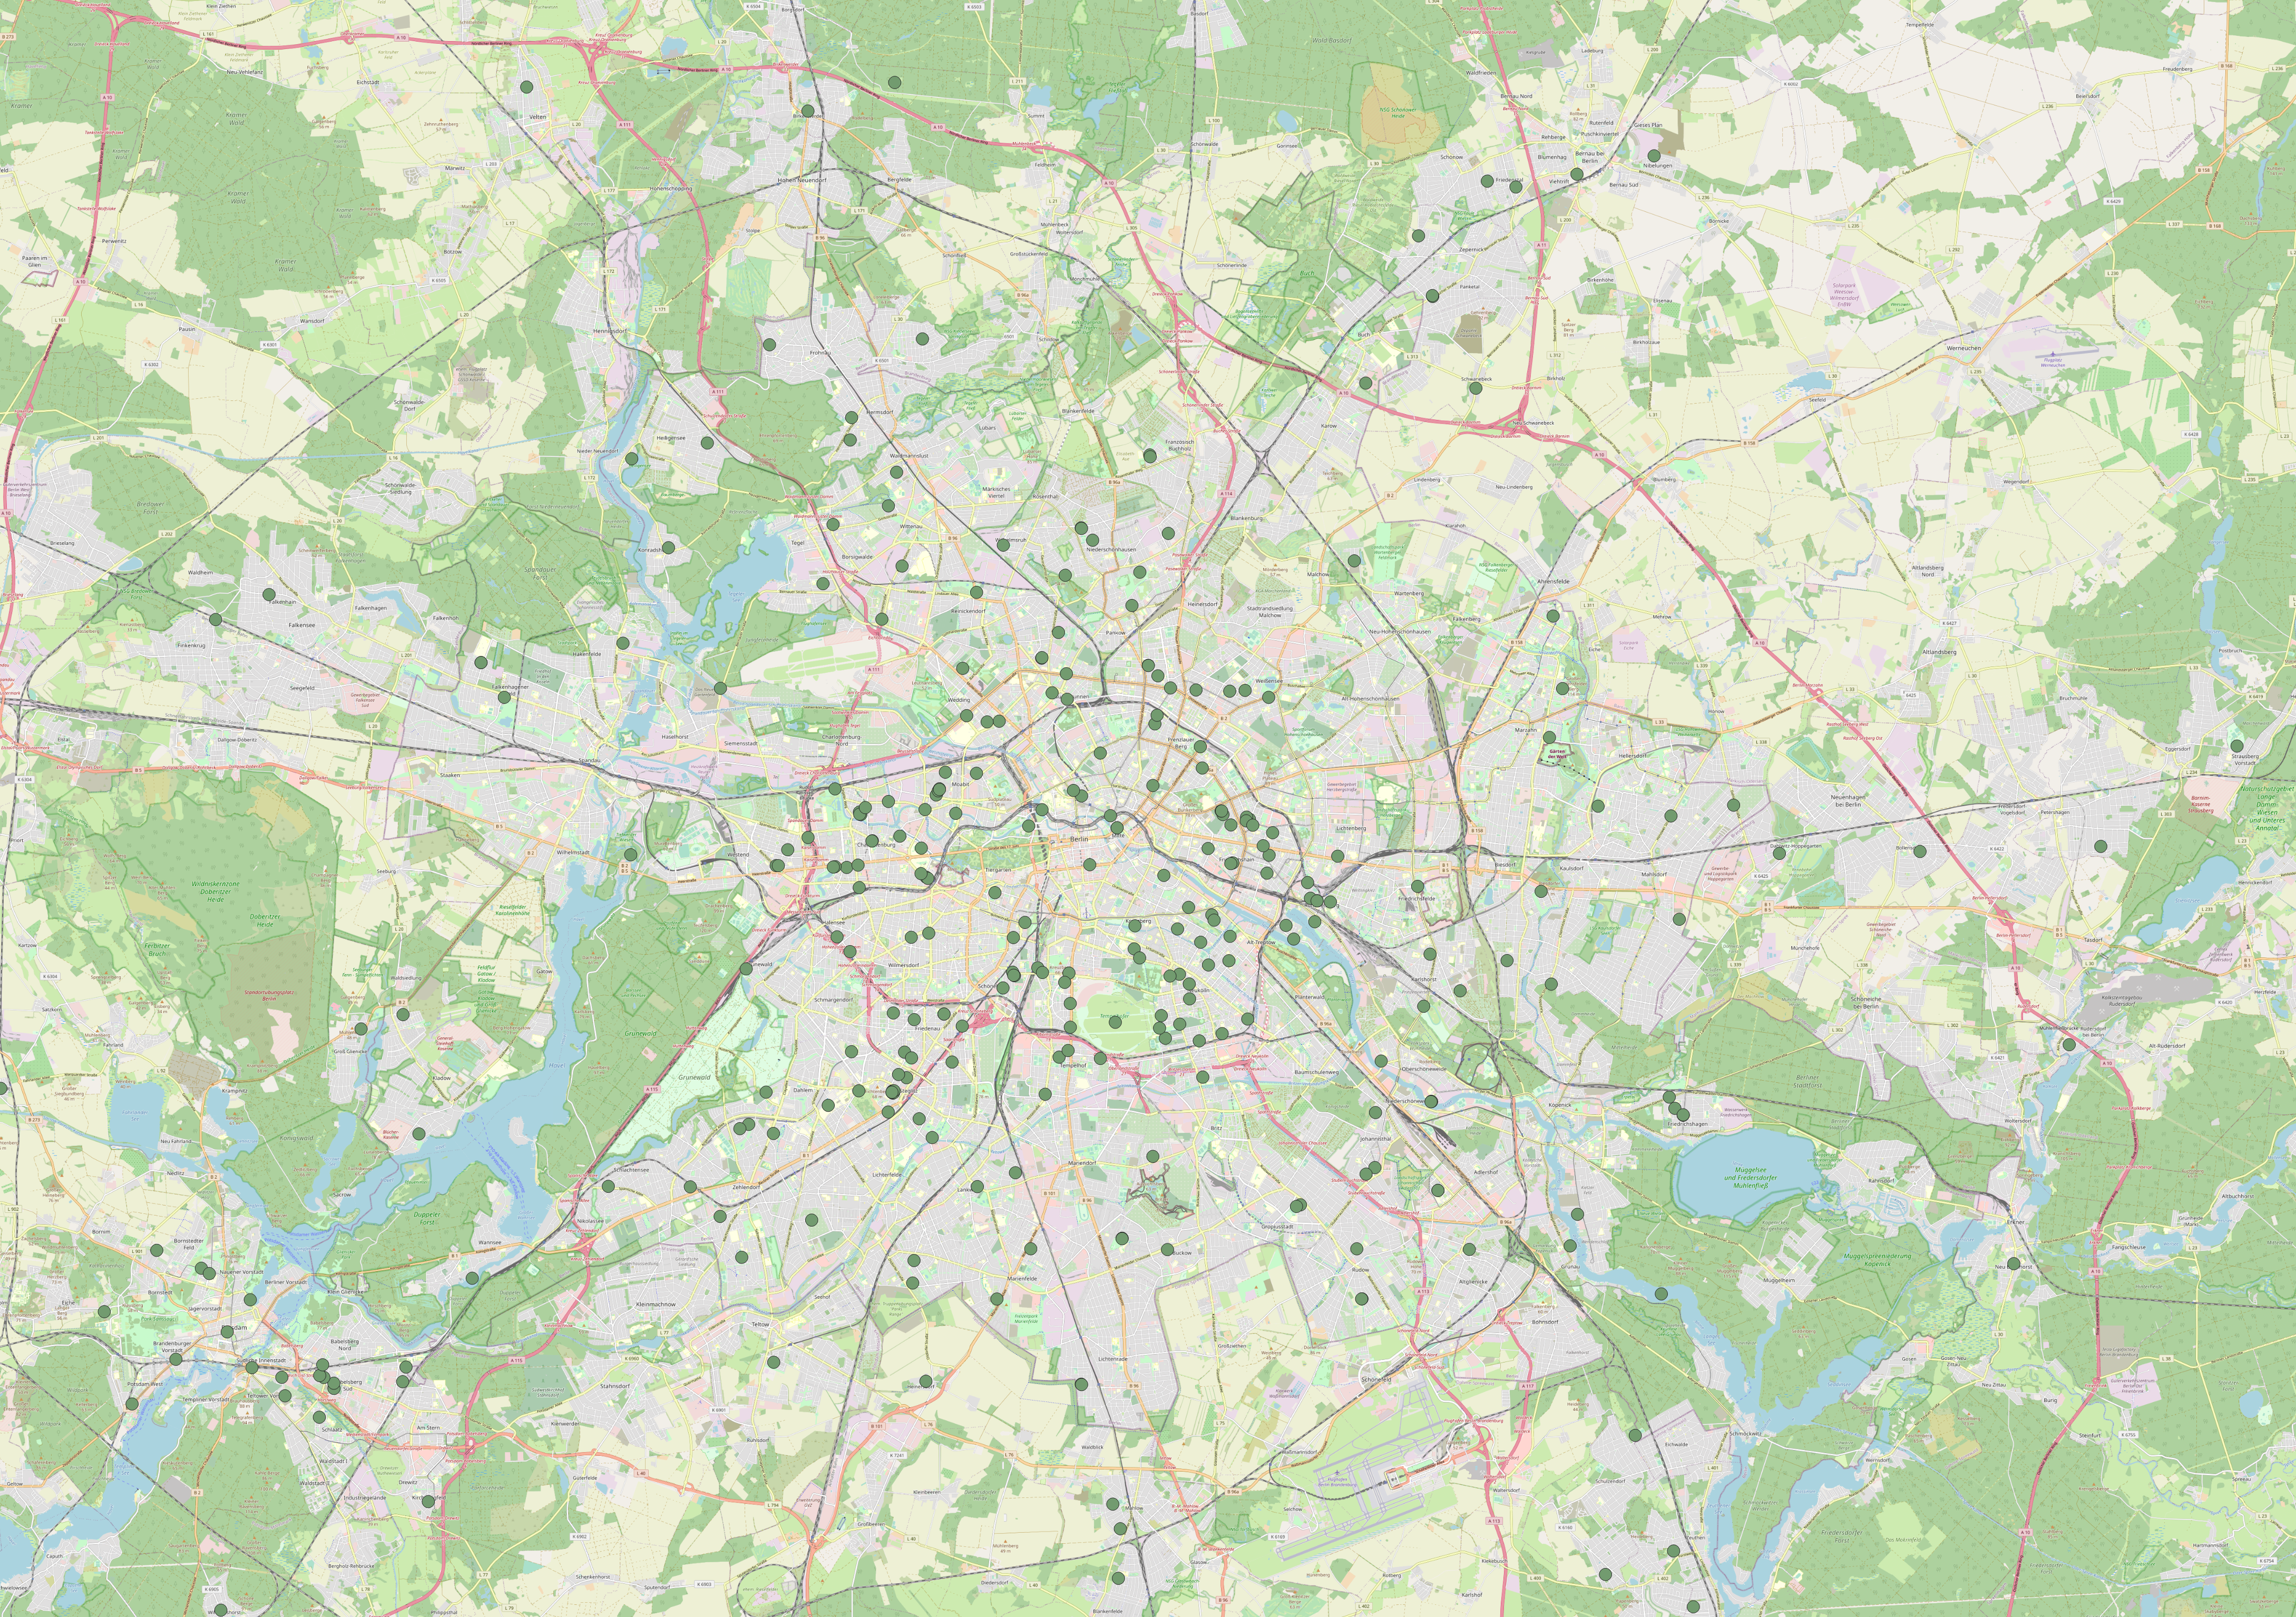
\includegraphics[width=.7\linewidth]{images/station_distribution.png}
	\caption{Distribution of sensor stations that measure the \ldq{}Temperatur\rdq{} phenomenon}
	\label{fig:station_dsitribution}
\end{figure}